\documentclass[final]{beamer} % beamer 3.10: do NOT use option hyperref={pdfpagelabels=false} !
% Began with this: https://tex.stackexchange.com/a/24266

\mode<presentation> {  %% check http://www-i6.informatik.rwth-aachen.de/~dreuw/latexbeamerposter.php for examples
  \usetheme{Berlin}    %% you should define your own theme e.g. for big headlines using your own logos 
%  \usetheme{metropolis}

}

\usepackage[english]{babel}
\usepackage[latin1]{inputenc}
\usepackage{amsmath,amsthm, amssymb, latexsym}
\usefonttheme[onlymath]{serif}
\boldmath
\usepackage[size=custom,width=116,height=106.5,scale=3]{beamerposter} % e.g. for custom size poster
\usepackage{graphicx}
%\usepackage{wrapfig}


\definecolor{forest_green}{RGB}{34,139,34}
\definecolor{usda_green}{RGB}{0,89,65}
%\setbeamercolor{title}{fg=forest_green}
%\setbeamercolor{frametitle}{fg=forest_green}
%\setbeamercolor{structure}{fg=forest_green}
\setbeamercolor{structure}{fg=usda_green}

\title[Detecting CNV with vcfR]{Detection of copy number variation for chromosomal sliding windows using high throughput sequencing data in the R environment}
\author[Knaus \& Gr\"unwald]{Brian J. Knaus and Niklaus J. Gr\"unwald}
\institute[USDA, ARS]{USDA, ARS, Horticultural Crops Research Unit}
\date{July 29th, 2018}

\setbeamertemplate{headline}{  
  \leavevmode

  \begin{beamercolorbox}[wd=\paperwidth]{headline}
    \begin{columns}[T]
      \begin{column}{.02\paperwidth}
      \end{column}
      \begin{column}{.7\paperwidth}
        \vskip8ex
        \raggedleft
        \usebeamercolor{title in headline}{\color{fg}\textbf{\large{\inserttitle}}\\[1ex]}
        \usebeamercolor{author in headline}{\color{fg}\normalsize{\insertauthor}\\[1ex]}
        \usebeamercolor{institute in headline}{\color{fg}\small{\insertinstitute}\\[1ex]}     
      \end{column}
      \begin{column}{.15\paperwidth}
        \vskip8ex
        \begin{center}
          \includegraphics[height=10cm]{./figures/usda-symbol.pdf}
          %Logo goes here.
        \end{center}
        \vskip2ex
      \end{column}
      \begin{column}{.02\paperwidth}
      \end{column}
    \end{columns}
    \vskip2ex
  \end{beamercolorbox}

  \begin{beamercolorbox}[wd=\paperwidth]{lower separation line head}
    \rule{0pt}{0pt}
  \end{beamercolorbox}
}
\setbeamertemplate{footline}{
  \begin{beamercolorbox}[wd=\paperwidth]{upper separation line foot}
    \rule{0pt}{3pt}
  \end{beamercolorbox}

  \leavevmode%
  \begin{beamercolorbox}[ht=4ex,leftskip=1em,rightskip=1em]{author in head/foot}%
    \texttt{http://grunwaldlab.cgrb.oregonstate.edu; https://doi.org/10.3389/fgene.2018.00123;  https://CRAN.R-project.org/package=vcfR}
    \hfill
    \texttt{Knaus and Gr\"unwald: CNV in vcfR}
    \vskip1ex
  \end{beamercolorbox}
  \vskip0pt%
  \begin{beamercolorbox}[wd=\paperwidth]{lower separation line foot}
    \rule{0pt}{3pt}
  \end{beamercolorbox}
}

\setbeamertemplate{navigation symbols}{}

\begin{document}
  \begin{frame}{}


    %%%%% %%%%% %%%%%
    %               %
    % New row       %
    %               %
    %%%%% %%%%% %%%%%
\begin{columns}[t]
  \begin{column}{0.44\textwidth}
    \begin{block}{\large Rationale}
%\small
\scriptsize
%\tiny
Inference of copy number variation presents a technical challenge because variant callers typically require the copy number of a genome or genomic region to be known a priori.
Our project required us to address this question, so we designed and implemented a method with the following:

\begin{itemize}
\item No a priori known base ploidy is required
\item Allows for genomic windows to be analyzed
\item Flexibility to use with non-model organisms
\item Works with VCF format data
\item Implemented in R
\end{itemize}

We validated these approaches with the model system of \textit{Saccharomyces cerevisiae}, an organism known to vary in ploidy and copy number.
This method has been implemented in the R package vcfR.
\vspace{3mm}
    \end{block}
  \end{column}

  \begin{column}{0.5\textwidth}
    \begin{block}{\large Chromosomal perspectives}
      \begin{columns}
        \begin{column}{0.4\textwidth}
%\small
%\footnotesize
\scriptsize
%\tiny
\\
\vspace{1mm}
%Different data types provide different perspectives.
Sequence depth can be used to characterize base ploidy and deviations from base ploidy.
However, if a research question includes 'what is base ploidy' we need another perspective.
Allele balance can help provide inferences on whether base ploidy is diploid, triploid, or tetraploid.
This is a reproduction of Figure 7 from Zhou et al. (2016) created in vcfR and highlights chromosome XII as having three copies while base ploidy is two copies.
%\vspace{2mm}
%          \begin{figure}
        \end{column}
        \begin{column}{0.55\textwidth}
          \includegraphics[height=20cm]{./figures/fig4_chrom_YJM1098.png}
        \end{column}
      \end{columns}
%          \caption{Allele balance is the frequency theat the most abundant and second most abundant allele were sequenced at.}
%          \end{figure}

    \end{block}
  \end{column}

\end{columns}




\vspace{5mm}


    %%%%% %%%%% %%%%%
    %               %
    % New row       %
    %               %
    %%%%% %%%%% %%%%%
\begin{columns}[t]
  \begin{column}{0.40\textwidth}
    \begin{block}{\large Depth and heterozygosity}
%\small

      \begin{columns}
        \begin{column}{0.45\textwidth}
          \includegraphics[height=8cm]{./figures/fig2_scer_dp_vplot.pdf}
          \newline
          \includegraphics[height=8cm]{./figures/fig3_scer_het_vplot.pdf}
        \end{column}
        \begin{column}{0.53\textwidth}
%\footnotesize
\scriptsize
\\
\vspace{10mm}
Here we summarize the per window sequencing depth and rate of heterozygosity throughhout \textit{S. cerevisiae} genomes.
This can be used to identify regions of the genome that are anomalous.
For example, we observe long tails of low heterozygosity that may be regions of lost heterozygosity.
\vspace{22mm}
        \end{column}
      \end{columns}

    \end{block}
  \end{column}

  \begin{column}{0.52\textwidth}
    \begin{block}{\large Allele balance}
      \begin{columns}
        \begin{column}{0.49\textwidth}
%\small
%\footnotesize
\scriptsize
%\tiny
\\
\vspace{1mm}
Allele balance is the frequency that the most abundant and second most abundant allele were sequenced at.
For diploids we expect half of the sequences to be from each allele.
For triploids we expect the alleles to be sequenced at frequencies of one thirds (1/3 and 2/3).
For tetraploids we expect the alleles to be sequenced at frequencies of quarters (1/4, 1/2, and 3/4).
This information can be used to assign a copy number to a genome or a genomic fraction.
%\vspace{20mm}
%          \begin{figure}
        \end{column}
        \begin{column}{0.4\textwidth}
          \includegraphics[height=14cm]{./figures/fig1_ab_example.pdf}
        \end{column}
      \end{columns}
%          \caption{Allele balance is the frequency theat the most abundant and second most abundant allele were sequenced at.}
%          \end{figure}

    \end{block}
  \end{column}


\end{columns}




\vspace{5mm}


    %%%%% %%%%% %%%%%
    %               %
    % New row       %
    %               %
    %%%%% %%%%% %%%%%
\begin{columns}[t]
  \begin{column}{0.71\textwidth}
    \begin{block}{\large A model for emergence}
      \begin{columns}
        \begin{column}{0.55\textwidth}
%\small
\footnotesize
%\tiny
Most emergences of \textit{P. infestans} may be ephemeral.
Occasional emergence of high fitness lineages displace preceding lineages.
Our work shows that these high fitness clones are also associated with high CNV.
This research also indicates a link between a copy number of two and a sexual mode of reproduction.
It is currently unknown whether a copy number of three drives fitness or it accumulates after highly fit lineages emerge.
It is also unknown if lineages of high copy number can revert back to a copy number of two.
        \end{column}
        \begin{column}{0.44\textwidth}
          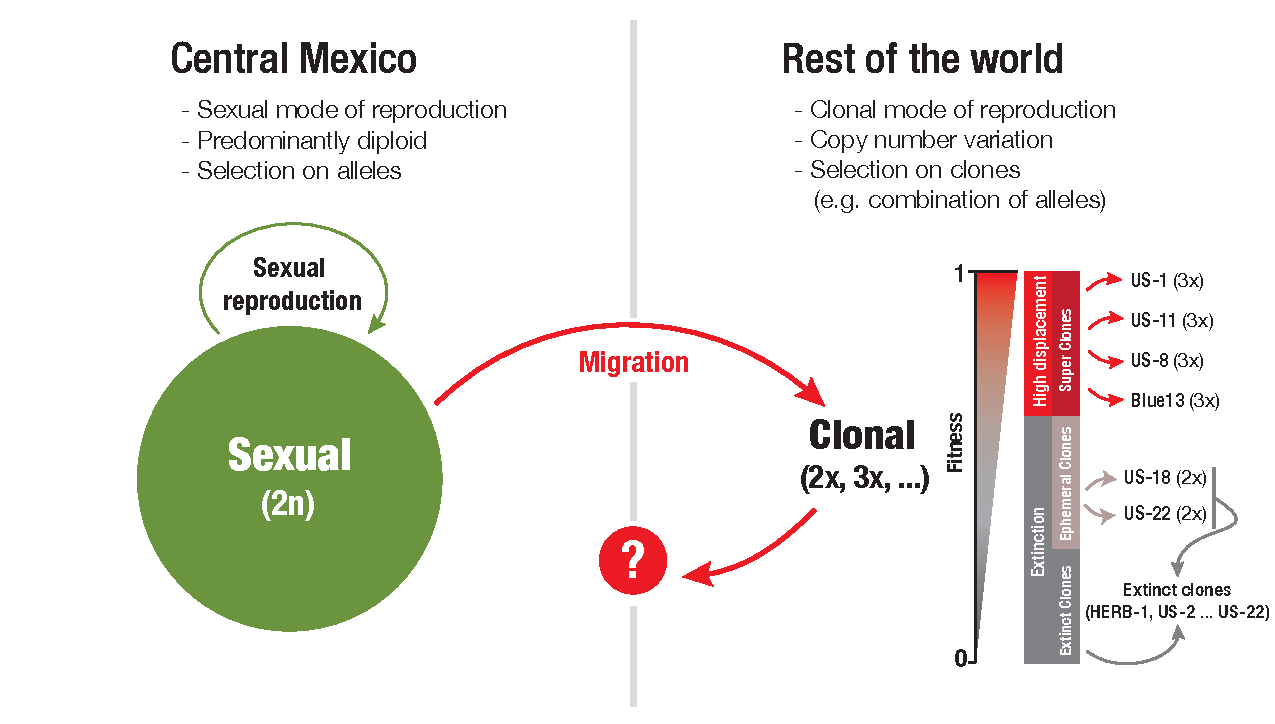
\includegraphics[height=20cm]{./figures/Fig8_Model.pdf}
        \end{column}
      \end{columns}

    \end{block}
  \end{column}

  \begin{column}{0.22\textwidth}
    \begin{block}{\large Acknowledgments}
\tiny
\vspace{10mm}

This research is supported in part by USDA National Institue of Food and Agriculture Grant 2011-68004-30154.
\newline
\vspace{5mm}

\textbf{References}\\
Knaus, B. J., \& Gr\"unwald, N. J. (2018). Inferring variation in copy number using high throughput sequencing data in R. Frontiers in Genetics, 9.
\newline
\vspace{1cm}

vcfR can be found at:
https://CRAN.R-project.org/package=vcfR
\vspace{1cm}

    \end{block}
  \end{column}
\end{columns}




  \end{frame}
\end{document}

